%%%%%%%%%%%%%%%%%%%%%%%%%%%%%%  IEEEsample2e.tex %%%%%%%%%%%%%%%%%%%%%%%%%%%%%%
%%%%%%%%%%%%%%%%%%%%%%%%%%%%%%  IEEEsample2e.tex %%%%%%%%%%%%%%%%%%%%%%%%%%%%%%
%%%%%%%%%%%%%%%%%%%%%%%%%%%%%%  IEEEsample2e.tex %%%%%%%%%%%%%%%%%%%%%%%%%%%%%%
%% changes for IEEEtrans.cls marked with !PN
%% except all occ. of IEEEtran.sty changed IEEEtran.cls
%%%%%%%%%%                                                       %%%%%%%%%%%%%
%%%%%%%%%%    More information: see the header of IEEEtran.cls   %%%%%%%%%%%%%
%%%%%%%%%%                                                       %%%%%%%%%%%%%
%%%%%%%%%%%%%%%%%%%%%%%%%%%%%%%%%%%%%%%%%%%%%%%%%%%%%%%%%%%%%%%%%%%%%%%%%%%%%%%


\documentclass[twocolumn]{IEEEtran} %!PN
%\documentclass[12pt,draft]{IEEEtran} %!PN
%\documentstyle[twocolumn]{IEEEtran}
%\documentstyle[12pt,twoside,draft]{IEEEtran}
%\documentstyle[9pt,twocolumn,technote,twoside]{IEEEtran}

\usepackage[section]{placeins}

\def\BibTeX{{\rm B\kern-.05em{\sc i\kern-.025em b}\kern-.08em
    T\kern-.1667em\lower.7ex\hbox{E}\kern-.125emX}}

\newtheorem{theorem}{Theorem}
\setcounter{page}{100}

\begin{document}

%\title{Using the Style File IEEEtran.sty} 
\title{A Novel Enhanced Radar on Software Define Radio} %!PN

\author{Bowen Song}

% \markboth{IEEE Transactions On Automatic Control, Vol. XX, No. Y, Month
% 1999}
%{Murray and Balemi: Using the style file IEEEtran.sty} %!PN
% {Murray and Balemi: Using the Document Class IEEEtran.cls} %!PN


\maketitle
%\thispagestyle{plain}\pagestyle{plain}

\begin{abstract}
This is an entrepreneur project to start off an affordable low power mobile radar software solution. This mobile Radar solution utilizes basic Software Defined Radio, low cost antennas, and home use computer. The foreseeable application applies to all drone controlled areas.\\

The software Radar solution uses a Linear Frequency Modulated waveform (LFM). It measures the object range and object speed by the Matched Filter and Moving Target Detection algorithms respectively. The main difference between our Radar and market available LFM Radar is the Digital Signal Processing algorithms and n-signal enhancements.\\

The project resulted in an accurate Radar system and is able to successfully detect nearby targets. Detecting fast moving objects is the strength of the Radar system, based on its waveform and the algorithms implemented. Because the project uses Software Defined Radio, other waveforms and algorithms can be used to further satisfy the requests of individual clients.
\end{abstract}

\begin{keywords}
LFM Radar, N-siganl, TC-OLA, DSP. 
\end{keywords}

\section{Introduction}
Software defined radio has been advancing the field of radio for several decades, making radio frequency devices cheaper and much more flexible than ever. By moving most of the radio system into the digital domain the work that was once done by a multitude of analog components is now done by embedded systems and general purpose processors. This allows for smaller, cheaper, and much more versatile system.\\

The entire Radar system is designed as software solution, applicable for variety of purposes. The product is compatible with most SDR hardware on the market. Depending on the budget of customers and their purpose, different combinations of hardware are recommended. Generally the system only requires a home use computer, a SDR, and an antenna. \\

The original market intent of this Radar solution was meant for companies that are already using Radar. Since the industry has yet to accept software Radar solution, this project offers an upgrade to existing Radar system. However, with the raise of popularities in drones, new regulation and enforcement for such technology is needed and desperate for near ground airspace management.\\

A perfect example comes from current abuse of UAV technology where criminals expands drone delivery to prison. Such behaviors pose as threats to public safety and law enforcement. Some governments have issued formal announcement addressing these type of crises such as the UK Ministry of Justice\cite{noauthor_uk_2016}. The current solutions involve training eagles and embedding no-fly zone program inside UAVs; these solutions do not eradicate drone problems. This project offers to equip prisons with affordable UAV Radars, detecting small fast approaching flying objects. The solution is efficient at alerting UAV entrance and within most government budget.\\

% \begin{figure}[h]
% \centering\makebox{\includegraphics[width=\textwidth]{droneprison}}
% \caption{Drone issue for prison security presented by UK Ministry of Justice\cite{noauthor_uk_2016}}
% \label{fig:droneprison}
% \end{figure}

With the true potential of UAVs yet to be realized in the civilian world, it is predicted that in the future our airspace will become much more cluttered. Managing the airspace of the future is expected to be a big business and organizations such as NASA, the FAA, Amazon, Google, Intel are already working on airspace solutions\cite{gipson_nasa_2017}. Small and inexpensive Radars like the product from this project will be a vital component of the airspace management systems of the future.
\section{Problem Definition}
\subsection{Project Scope}
This mobile inexpensive Radar project is focusing on designing compatible software that runs on home use laptops and transceives with affordable SDRs and antennas. The software solution includes traditional LFM Radar with Digital Signal Processing (DSP) and n-signal enhancement. The DSP improvement is increasing the Signal to Noise Ratio (SNR) and spectrum of the bandwidth. The two increments are sustaining the high detection rate at poor signal reception and with presence of regular jamming signal respectively. The n-signal enhancement is to allow Radar to be multi-purposed. Every waveform has its strengths and weaknesses; n-signal is a way to integrate multiple waveforms with their unique properties into one signal for Radar to fit under multiple purposes. The project lists out general hardware requirements and specifications according to the recommended hardware packages, Appendix \ref{app:specs}. 
\subsection{Problem Approach}
There are two main platforms to develop the software for the Radar system, MATLAB-Simulink and GNURadio. Both platforms offers graphical environment for simulating and analyzing dynamic systems. While Simulink offers vast amount of integrated native algorithms and image rendering, its USRP communication block contains fatal error disregarding transceiving sample time, which is discussed in Appendix \ref{app:simuerror}. On the contrary, GNURadio is respectful to transceiving data and sample time while provides less native algorithms and less comprehensible data display. Therefore, this project integrates the best from each platform, having GNURadio to transceive signals and MATLAB-Simulink to deliver final result. 
\subsection{Project Goal}
The product of this project is set to demonstrate the ability to manage near ground airspace. Due to project budget limits, the project will only concern activities within capabilities of 18-elements Yagi antennas and USRP N210. More versions that best fit other Radar purposes can be done under client request. 


\section{Radar Technology And Design Choices}
Due to the inherited software nature, Radar implemented on SDR is able to select wild range of signal processing methods to add on to the existing system. This section explains traditional LFM Radar components and the two enhancements upon the implementation.
%-------------------------------------------------------------------------------
% LFM
%-------------------------------------------------------------------------------
\subsection{LFM Radar implementing on SDR}
According to the product market intention for airspace management, Linear Frequency Modulated waveform is chosen for its ability to capture high speed object due to its tolerance for Doppler shift. The Doppler shift is a result of object moving; as the object moves faster, the bigger the Doppler shift. The Radar system includes Matched Filter, MTD, and CFAR in its receiver, system flow graph shown in Figure \ref{fig:LFMcomp}. Each component is responsible for ranging, speed measuring, and deciding noise floor threshold accordingly. The use of Yagi directional antenna is acting as a stationary Radar antenna. For an airspace managing Radar, antenna is not stationary and a rotation synchronization to the software system is needed. The Mimo Cable in between the two USRPs is a way to synchronize two SDRs. \\
\begin{figure}[h]
{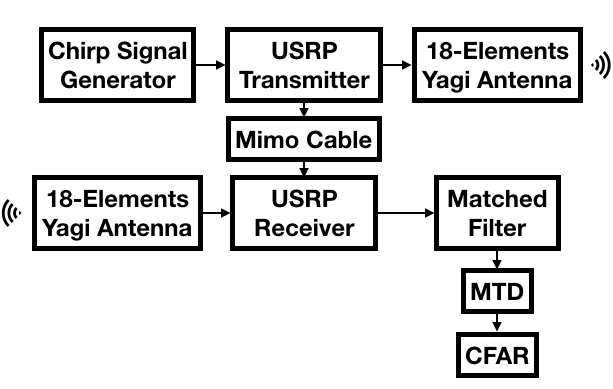
\includegraphics[width=\textwidth]{LFMcomp.png}}
\caption{LFM Radar system flow graph}
\label{fig:LFMcomp}
\end{figure}
\FloatBarrier
% \subsubsection{Matched Filter}
% Matched Filter (MF) is the ranging component of the Radar. It convolves received signal with reverse conjugate of the transmitted signal. Since there are embedded patterns that differentiate the signal from surrounding signals and noise, Matched Filter is able to pick up only the useful information. The matched filter presents tanging information by showing peaks. The time distance between the peaks gives out the time frame between signal transiting from antenna and signal reception after bouncing back from target object. The Radar system uses antenna side lobe signal to mark transmitting time stamp, since the receiving antenna captures side lobe signal almost instantly after transmission. In the system, the side lobe signal traveled distance is taking from total measured range to get accurate result. Figure \ref{fig:mfex} provides an example of LFM signal before transmission, after receiver, and its matched filter result. A further explanation can be found in Appendix \ref{app:tdmf}.
% \begin{figure}[h]
% \centering\makebox{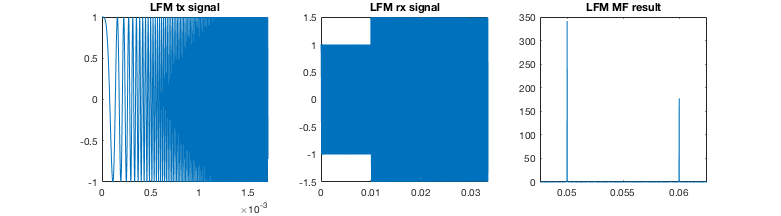
\includegraphics[width=\textwidth]{mfex.png}}
% \caption{Tx signal pattern, rx signal with 0.01 s delay from transmission time stamp, and MF result}
% \label{fig:mfex}
% \end{figure}
% \FloatBarrier
% \subsubsection{Moving Target Detection}
% Moving Target Detection (MTD) is the way to measure the speed of moving target. After detecting an object, MTD measures the Doppler shift in the received signal in comparing with the transmitted signal. The frequency difference is between the two peaks that provides the speed information of the moving object.

% \subsubsection{Constant False Alarm Rate}
% CFAR is used to set a threshold for peak detection. From matched filter output, a series of peaks are providing target distance, Radar system only counts the peaks that stands out from noise peaks. CFAR algorithm determines the threshold for the system to regard peaks as either noise or target and generates result in Figure \ref{fig:th} (left) instead of Figure \ref{fig:th} (right) which has threshold set lower than noise level and end up with too many peaks counted as target.
% \begin{figure}[h]
% \noindent\makebox{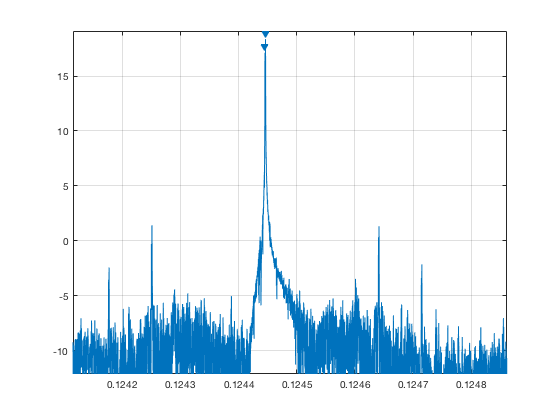
\includegraphics[width=0.5\textwidth]{th.png}}
% \noindent\makebox{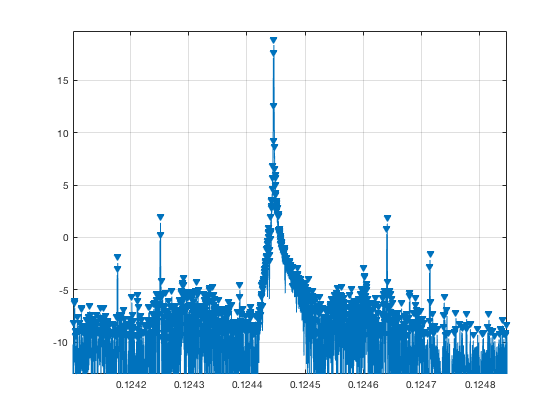
\includegraphics[width=0.5\textwidth]{lowth.png}}
% \caption{Matched filter result with peak detection}
% \label{fig:th}
% \end{figure}
% \FloatBarrier

% %-------------------------------------------------------------------------------
% %TCOLA
% %-------------------------------------------------------------------------------
% \subsection{Time Compression Overlap Add - DSP Enhancement}
% Working with software defined radio gives us great flexibility in the design of our Radar. We can take full advantage of complex signal processing techniques to make design trade-offs. \\

% A process that has been the topic of study at UVic is TC-OLA or Time Compression - Overlap Add. By adding this module to our design we can improve the signal processing gain and robustness of our Radar design. This module transforms the LFM chirp signal by dividing it up and transmitting the signal with redundancies. By adding this signal back together with the redundancies added a gain is seen at the receiver.\\

% By adding Time Compression - Overlap Add (TC-OLA) to our Radar design we can increase processing gain and the robustness of our Radar without change to the Doppler shift or target time delay of our pulse. TC-OLA consists of two modules, one at the transmitter to modify the sent pulses and one at the receiver to recover the original signal. The transmitted signal is divided into overlapping segments and sent sequentially, shown in Figure \ref{fig:tcola}. This DSP Processes is added to the system as shown in Figure \ref{fig:tcolafg}\\
% \begin{figure}[h]
% \centering\makebox{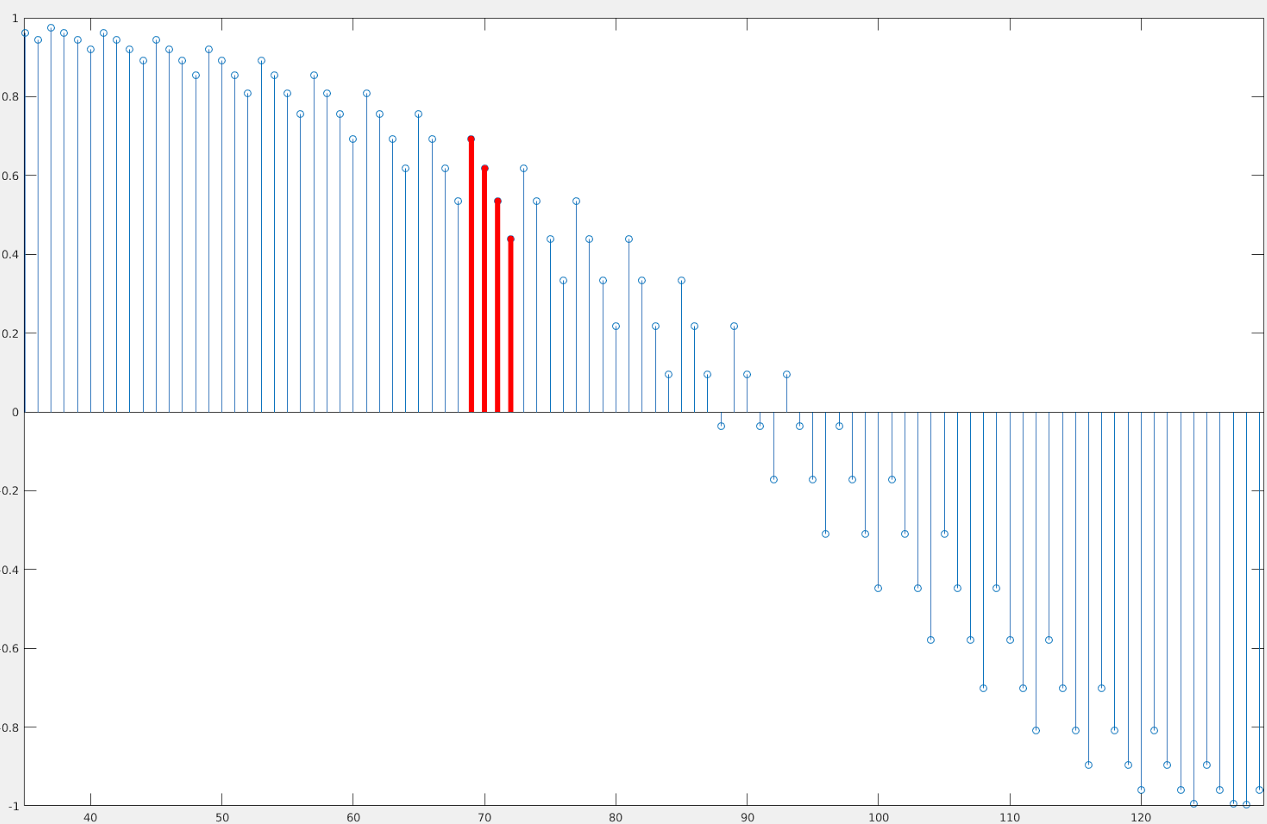
\includegraphics[width=0.5\textwidth,height = 4.1cm]{tcoladis.png}}
% \caption{LFM chirp signal modified by TC-OLA}
% \label{fig:tcola}
% \end{figure}
% \begin{figure}[h]
% \centering\makebox{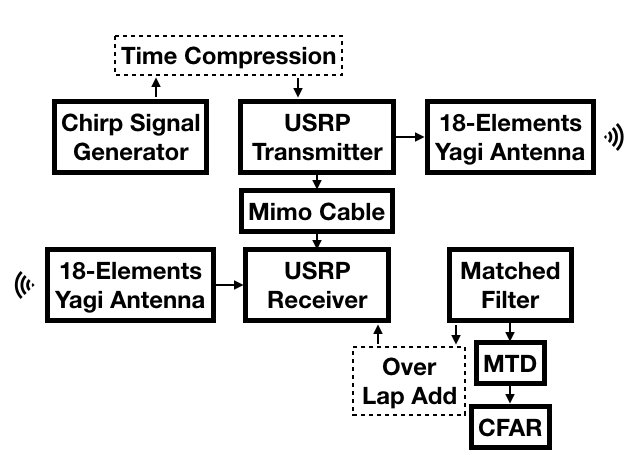
\includegraphics[width=0.5\textwidth]{tcolaflowg.png}}
% \caption{Radar system flow graph with DSP enhancement}
% \label{fig:tcolafg}
% \end{figure}
% \FloatBarrier
% \subsubsection{Time Compression}
% At the transmitter the time compression module is added. This takes the LFM signal and uses a sliding window to divide it into overlapping segments and then send the segments sequentially. Since the signal is compressed in time with abrupt changes in phase the TC-OLA signal will have higher bandwidth and therefore need a higher sampling rate ADC. 
% \subsubsection{Overlap Add}
% At the receiver the signal is uncompressed and the redundancy is turned into processing gain. To recover the original signal the received signal is partitioned, shifted by the original amount of overlap and then the sum of these segments is found.
% \subsubsection{Contribution to Project}
% By adding TC-OLA modules to our Radar system we get the benefit of higher processing gain, boosted signal to noise ratio and better immunity to interfering signals such as jamming (since the signal is spread over a larger bandwidth a jammer would need to use much more power). However as is common in design these advantages come at a price. TC-OLA requires greater bandwidth and higher processing rates than conventional LFM. This increases the overall cost of Radar system.

% %-------------------------------------------------------------------------------
% % N-Signals
% %-------------------------------------------------------------------------------
% \subsection{N-Signals Enhancement}
% The n-signal enhancement is a waveform modifying scheme derived from TC-OLA. This scheme takes different waveforms with same pulse duration and combines them into one signal. On the receiver end, a decoder extracts different waveforms out and match them with their own matched filter; flow graph shown in Figure \ref{fig:nsigfg}.
% \begin{figure}[h]
% \centering\makebox{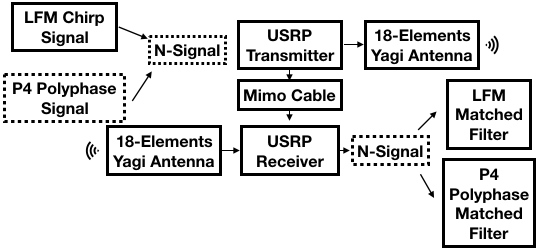
\includegraphics[width=0.5\textwidth]{nsigfg}}
% \caption{N-Signal flow graph}
% \label{fig:nsigfg}
% \end{figure}

% The n-signal scheme provides one fused signal for transmission and extract clean sub-signals from the fused signal. Figure \ref{fig:lfmBW2Nsq} shows the signals before been combined by the n-signal scheme on the left section, the fused signal for transmission through USRPs in the middle, and the signals after been extracted by the n-signal scheme on the right section. 
% \begin{figure}[h]
% \noindent\makebox{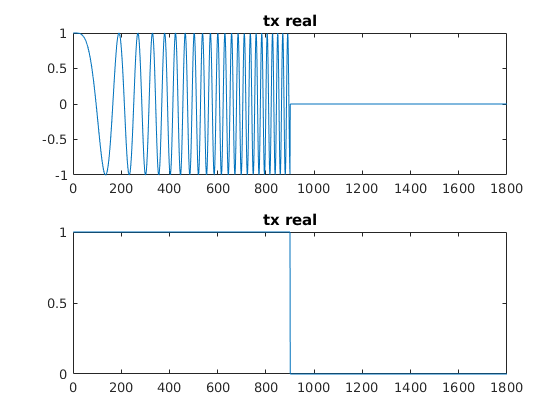
\includegraphics[width=0.33\textwidth]{nsig1}}
% \noindent\makebox{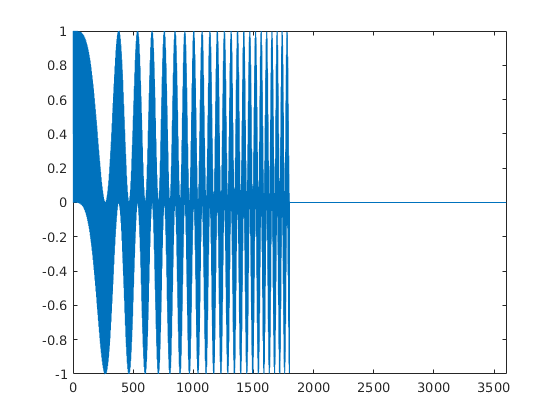
\includegraphics[width=0.33\textwidth]{nsiginter}}
% \noindent\makebox{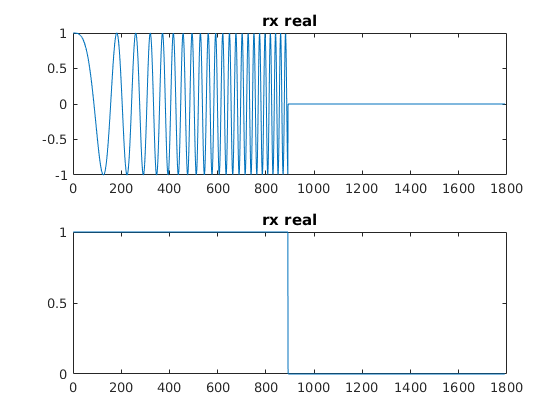
\includegraphics[width=0.33\textwidth]{nsig2}}
% \caption{LFM and square signals going through N-Signal scheme}
% \label{fig:lfmBW2Nsq}
% \end{figure}
% \FloatBarrier 
% %-------------------------------------------------------------------------------
% % Implementation and Experimentation
% %-------------------------------------------------------------------------------
% \newpage
% \section{Implementation And Experiments}
% Experiments are conducted repeatedly against different Radar software systems. This section contains two hardware setups, one of the most stable software implementation, and 
% \subsection{Hardware Experimental Setups}
% \begin{figure}[h]
% \centering\makebox{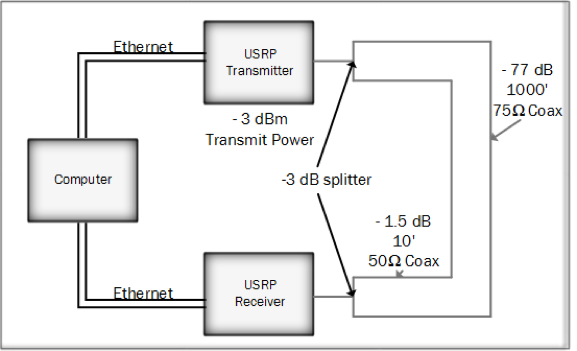
\includegraphics[width=0.5\textwidth]{cableex}}
% \caption{Simulated delay using 1000 feet cable}
% \label{fig:cableex}
% \end{figure}
% \[P_{R-short/coax}=-33dB-3dB-3dB-1.5dB= -40.5dB\]
% \[P_{R-long/coax}=-33dB-3dB-3dB-77dB= -116dB\]

% The Figure \ref{fig:cableex} setup was used to determine if the software portion of the radio was working by simulating the free space transmission path with a long cable that has less loss and a propagation delay.
% \begin{figure}[h]
% \noindent\makebox{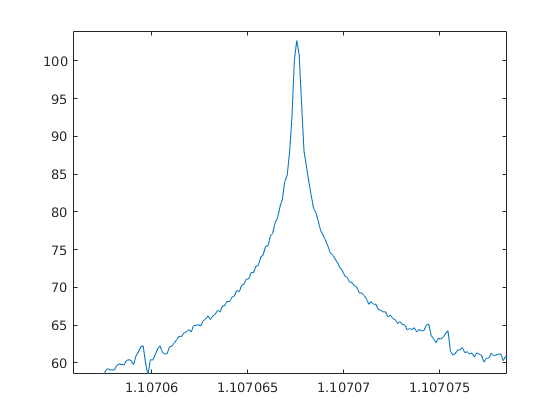
\includegraphics[width=0.5\textwidth]{one}}
% \noindent\makebox{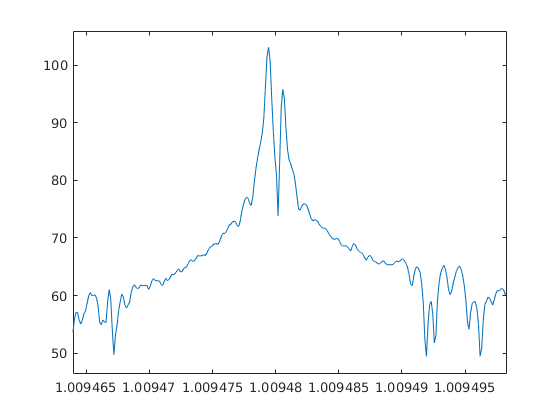
\includegraphics[width=0.5\textwidth]{ms80}}
% \caption{Receiver matched signal (left) with 1 coax, (right) with 2 coax connected and shorter cable attenuated}
% \label{fig:oneandms80}
% \end{figure}
% Figure \ref{fig:oneandms80} (left) has 1 signal, which is expected, at the receiving FFT. Figure \ref{fig:oneandms80} (right) shows two signals, one on from the short cable and one from the long cable. The time difference between these peaks is the length of the difference between these cables.
% \[Cable Length = VF*c*time = 0.81 * 3e8*1.25us = 303.75m\]
% The result is exactly what is expected, the source of error is the result of the time being measured and the actual propagation velocity though the cable being a close approximation.

% \begin{figure}[h]
% \centering\makebox{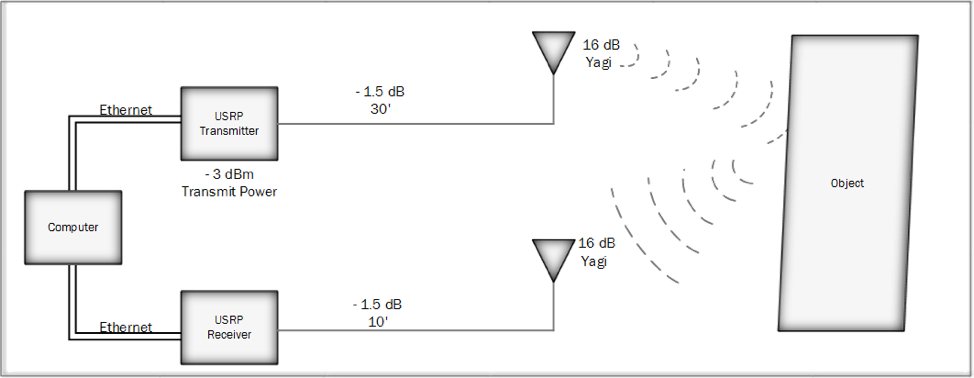
\includegraphics[width=\textwidth]{towerex}}
% \caption{Experimental Setup}
% \label{fig:towerex}
% \end{figure}

% Link Loss for transmission through air assuming 200m target: 
% \[P_{R} = -33dB-1.5dB+16dB-147.55dB+20log(200m)+20log900+16dB-1.5dB = -46dB.\]
 
% The hardware involved in this experiment was minimal because the focus is to use software to define this radio. However, a transmitter and separate receiver is used to keep things modular. Short cables are chosen with very little loss to go between the radios and the antenna because of the limited transmitter power (measured at -3dBm even though the spec sheet says 15 dBm). Finally, two high gain 18 element Yagi antennas are used for both transmitting and receiving. The received signal should be at -46 dB, which is enough for the receiver to detect easily.

% \subsection{GNURadio Implementation}
% As a successful attempt to implement the LFM Radar algorithm, the software GNURadio was selected as the interface for transmitting and receiving with the USRP N210.  GNURadio was used as the alternative to Simulink for its proven capability interfacing with the USRP hardware. The code initially developed for generating the LFM pulse modulated Radar signal had been developed using MATLAB. GNURadio supported the re-use of the chirp signals generated in MATLAB, exporting the results to a .wav file usable as the signal source for transmitting in GNU Radio. Similarly, the received Radar signal is saved using a file sink block as a .wav file for processing with MATLAB code. Figure \ref{fig:gnufgsimp} shows the flow graph used for transmitting and receiving the LFM Radar signals.
% \newline
% \begin{figure}[h]
% \centering\makebox{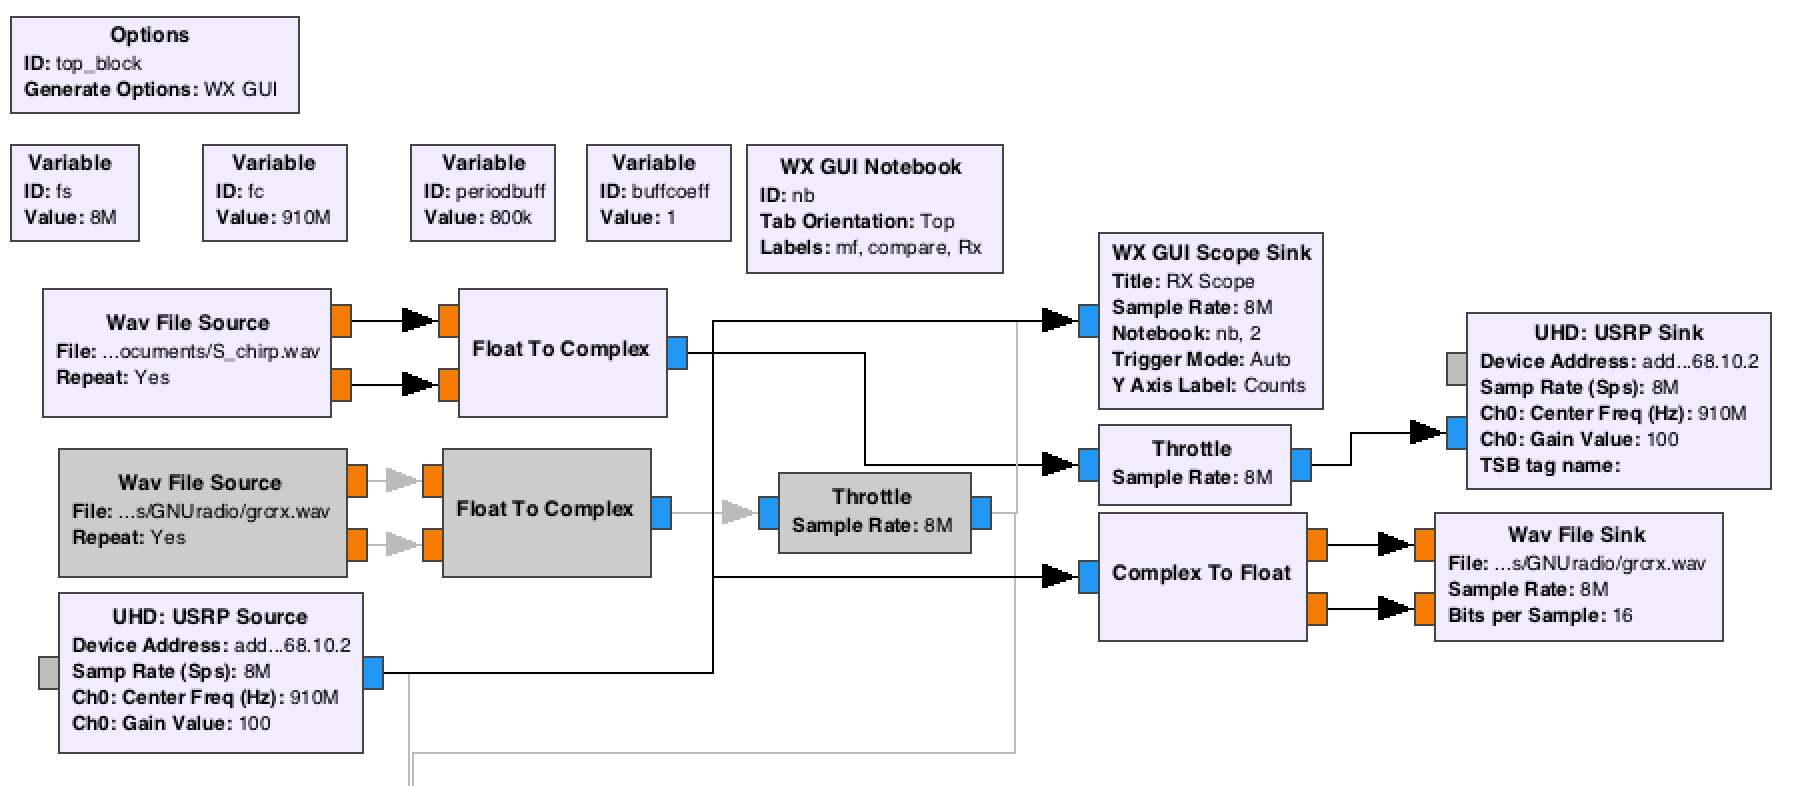
\includegraphics[width=0.5\textwidth]{gnufgsimp}}
% \caption{general view of GNURadio transceiver block diagram}
% \label{fig:gnufgsimp}
% \end{figure}

% The implementation in Figure \ref{fig:gnufgsimp} does not allow for real-time processing of the experimental Radar data. It simply transmits and receives the LFM Radar chirp signal. The file source and USRP sink block must be separated by a throttle block to limit CPU resource expenditure.  

% \subsection{LFM Radar Experimental Results}
% The experiment was a success, accurately computing distances to various nearby objects. The images and figures below are proof of correct Radar operation.\\
% \newline
% Figure \ref{fig:dome} (left) shows the distance from the antenna to the dome building, according to Google maps is 262.87m to travel the total distance. The Figure \ref{fig:dome} (right) shows the sent and received Radar pulses. The distance measured from the pulses between the peaks is 262.5m for the round trip distance. The marginal difference may be the result of side lobe travel time and human error on placing the exact locations of antennas and target object on Google map.\\

% \begin{figure}[h]
% \centering\makebox{
% \noindent\makebox{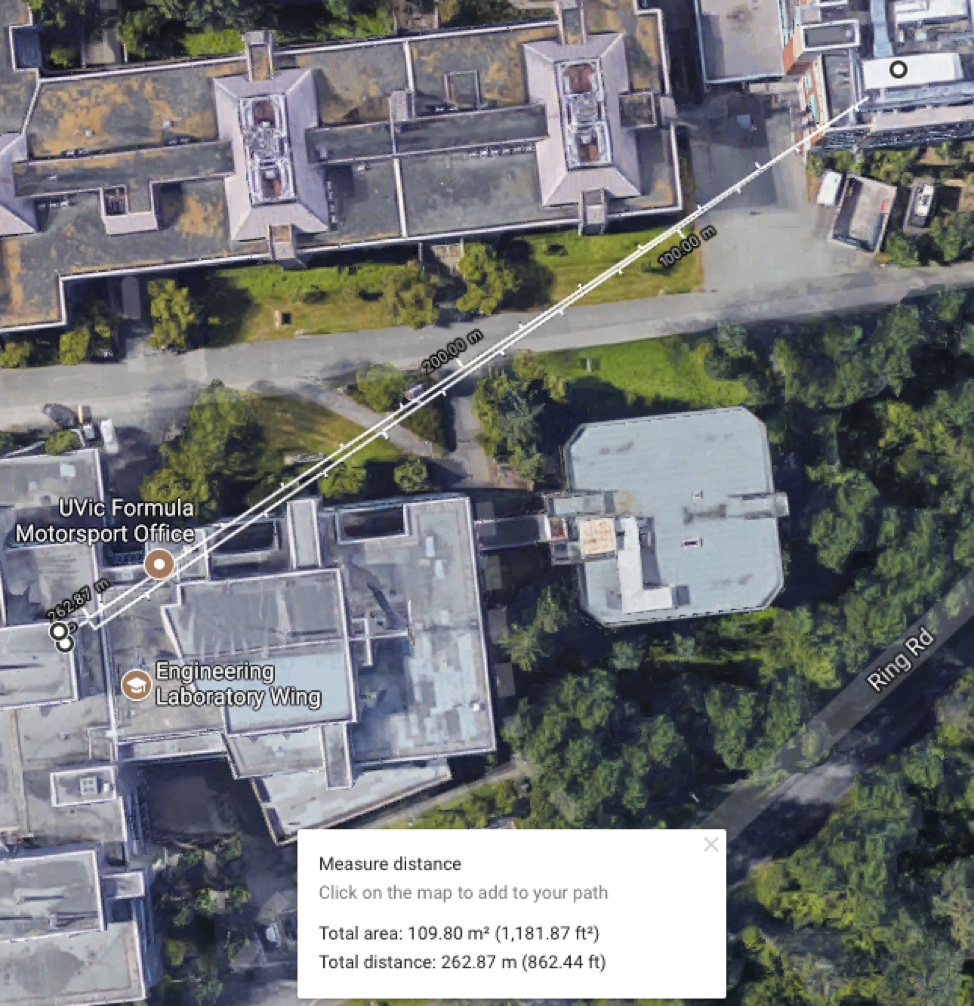
\includegraphics[width=0.335\textwidth]{domegoogle}}
% \noindent\makebox{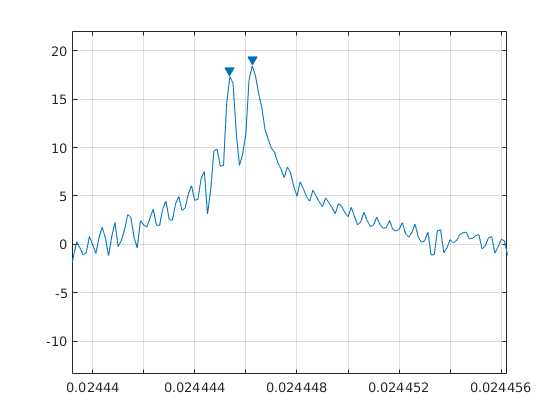
\includegraphics[width=0.45\textwidth]{domenear}}
% }
% \caption{Nearby dome building range measured by Google Map (left) and by Radar (right)}
% \label{fig:dome}
% \end{figure}
% \FloatBarrier
% For an alternative target, Figure \ref{fig:midtower} (left) shows the distance from the antenna to the smoke stack to be 100m on Google map. With previously stated uncertainty in the result still involved, the distance measured by our Radar is exactly 100m, and the corresponding sent and received pulses are shown in Figure \ref{fig:midtower} (right).

% \begin{figure}[h]
% \centering\makebox{
% \noindent\makebox{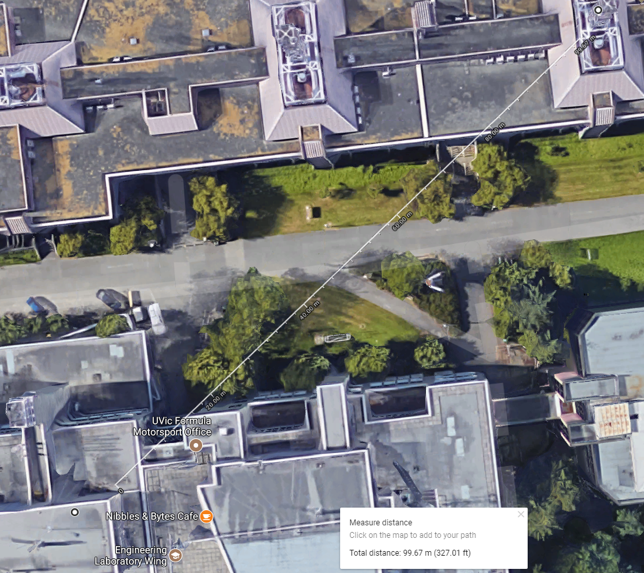
\includegraphics[width=0.335\textwidth]{midtowergoogle}}
% \noindent\makebox{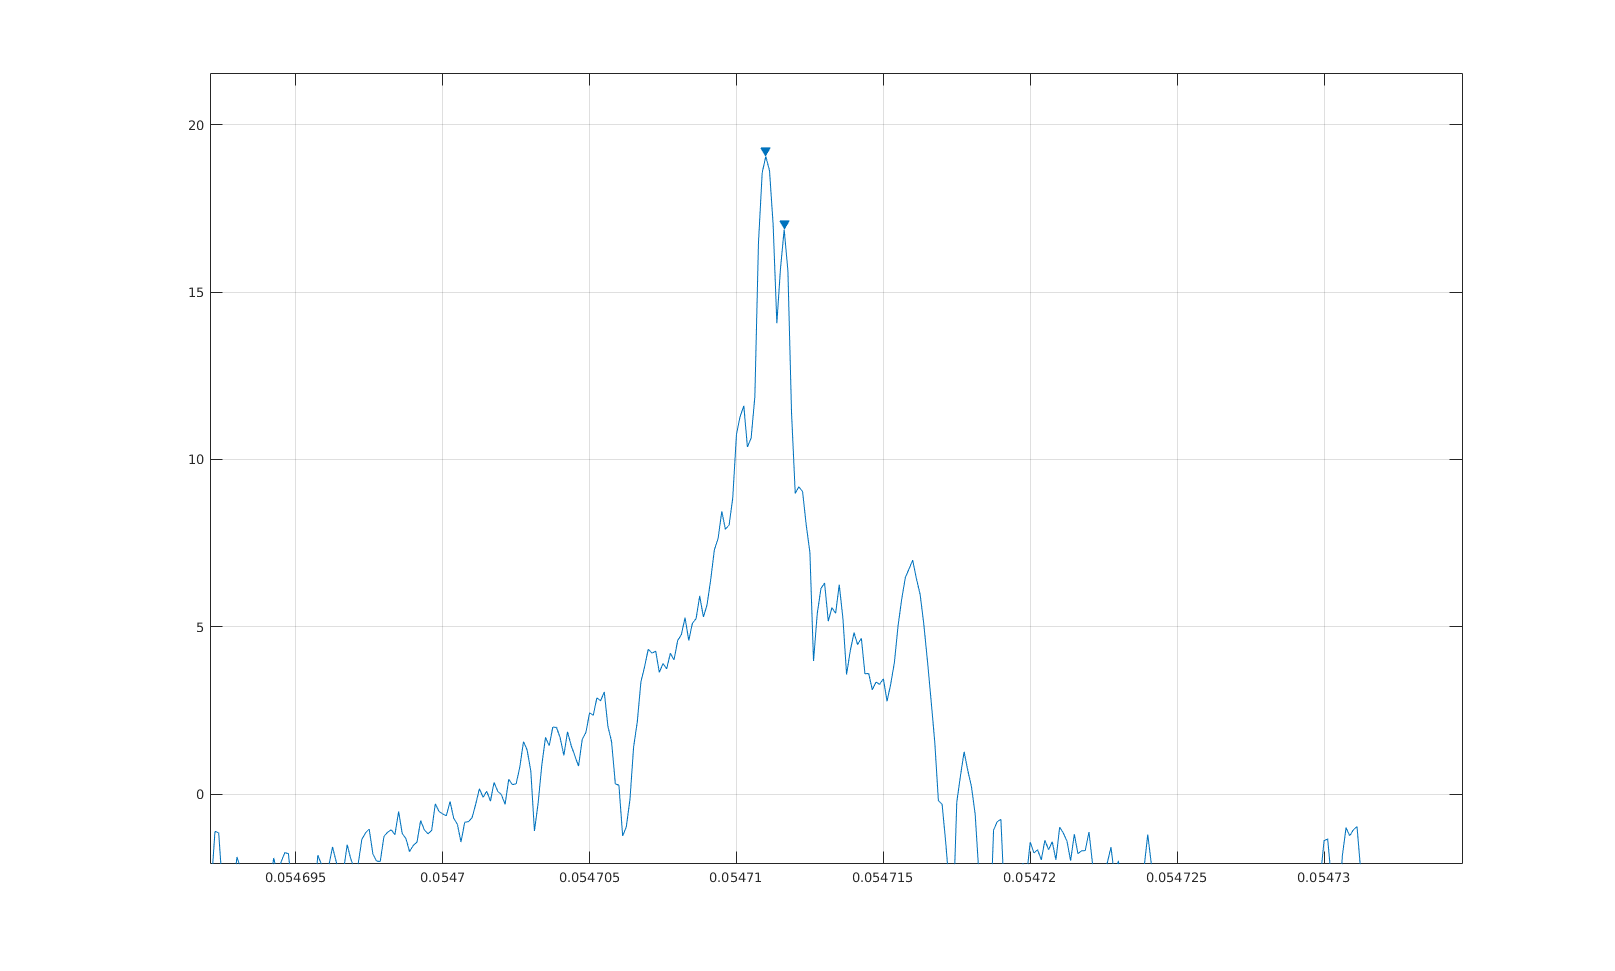
\includegraphics[width=0.5\textwidth]{roof200mnear}}
% }
% \caption{Nearby smoke stack building range measured by Google Map (left) and by Radar (right)}
% \label{fig:midtower}
% \end{figure}
% \FloatBarrier
% \subsection{TC-OLA Enhanced LFM Radar Experimental Results}
% An other series of tests based on the same hardware setups were performed on the Radar system. Due to hardware constrain, Radar system testing is only capable of detecting further away targets. For detecting near by target, hardware should be capable of transmitting signal with higher bandwidth, detailed explanation for the requirement of high bandwidth is presented in Appendix \ref{app:minDR}. \\
% \begin{figure}[h]
% \centering\makebox{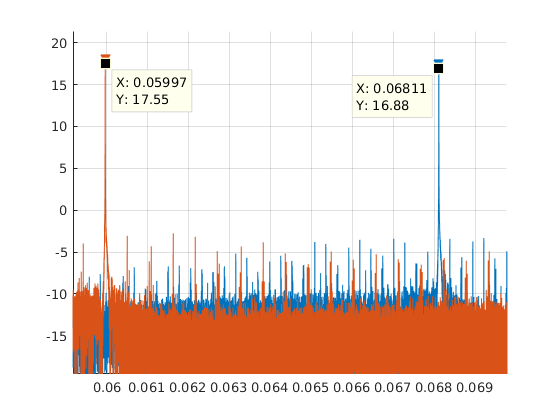
\includegraphics[width=0.5\textwidth]{Compare.png}}
% \caption{Comparing traditional (blue) with improved result(orange)}
% \label{fig:comp}
% \end{figure}

% The signal transfers through the experimental setups listed in Figure \ref{fig:towerex} and the matched filter result is overlaid on top of LFM Radar result without an enhancement. This is to compare the normal LFM result from improved results. A dB vs time graph is shown in Figure \ref{fig:comp}. This is considered to reflect  The TC-OLA, due to hardware constraint, is only able to double the gain and result in a 3 dB raise in SNR. The raise of at least 1 dB up indicates a great change in magnitude and matches the theoretical assumption.
% \FloatBarrier
% \subsection{N-Signal Enhanced Radar Experimental Results}
% The n-signal enhancement is tested against different combination of signal waveforms. The unique combinations are listed here from transceiving through the experimental setups listed in Figure \ref{fig:towerex}. The combinations includes different bandwidth LFM, LFM and Frank P4 polyphase, and LFM with square pulse.\\

% N-signals combining two LFM signals with different bandwidth and spectrum spreads the spectrum of the radar signal and increases jamming difficulties. Figure \ref{fig:lfmnlfm} shows the two LFM signals before combining by n-signal scheme on the upper section and after getting extracted from the received signal in the middle. The bottom section shows their matched filter result accordingly. The LFM signal on the left side has the bandwidth of $2 MHz$ where as the signal on the right has the bandwidth of $1 MHz$. While measuring the object that is 150 meters away, only the LFM signal with bandwidth of $2 MHz$ has the special resolution to show the second peak in the matched filter. This is presented by the peak finding algorithm in the bottom section of Figure \ref{fig:lfmnlfm}; notice by comparing the MF result, the LFM with bandwidth of $1 MHz$ shows the second peak fading in to the other peak due to lack of resolution. The result shows, even thought transmitted as one signal, n-signal combines the signals in a way that has different waveform within the fused signal distinctively targeting their own goals.\\

% \begin{figure}[h]
% \noindent\makebox{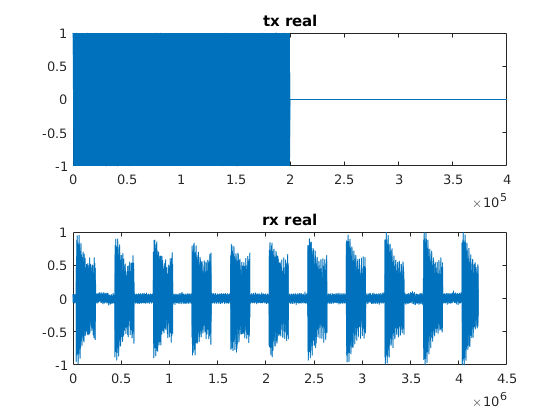
\includegraphics[width=0.5\textwidth]{txrxlfmb2ext1.png}}
% \noindent\makebox{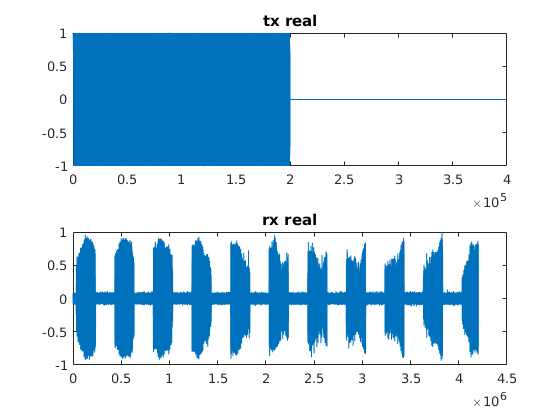
\includegraphics[width=0.5\textwidth]{txrxlfmb1ext2.png}}
% \noindent\makebox{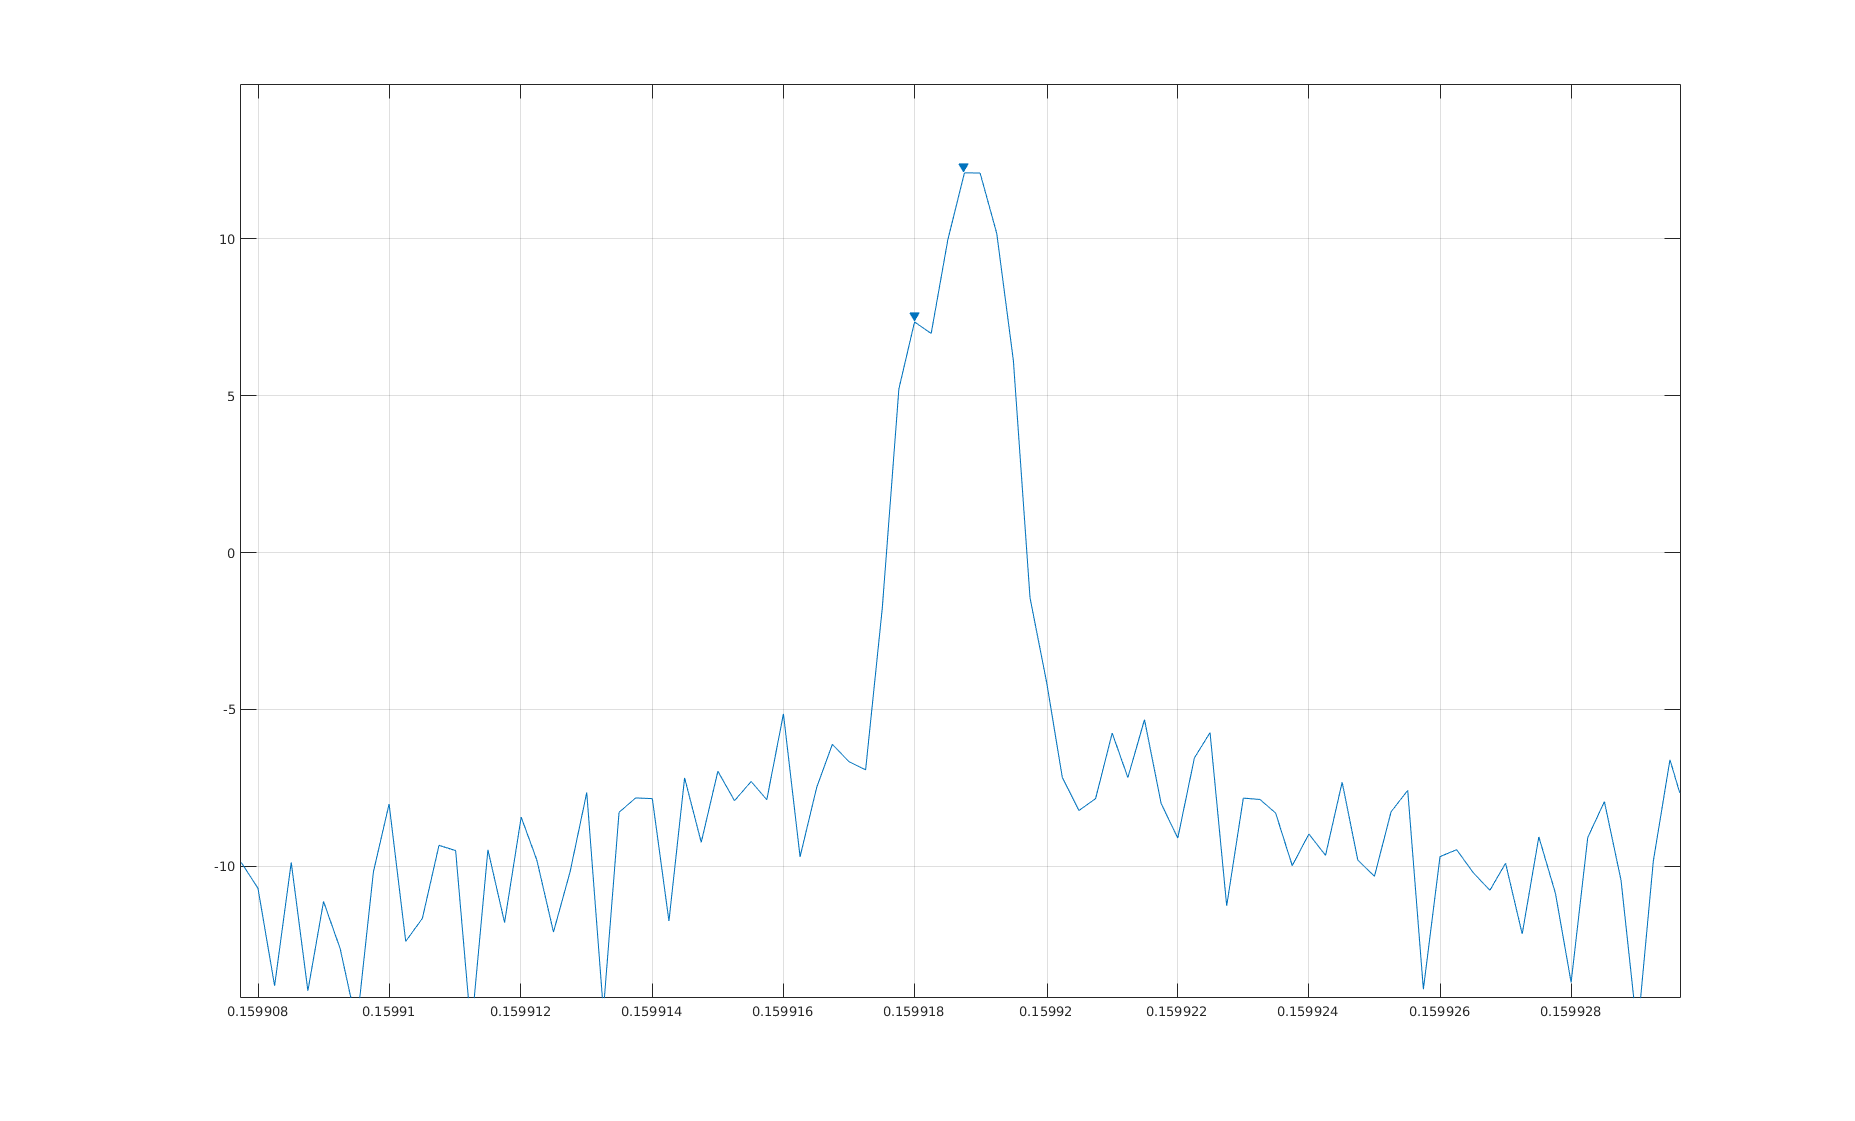
\includegraphics[width=0.5\textwidth,height=3cm]{LFMnsigwin3.png}}
% \noindent\makebox{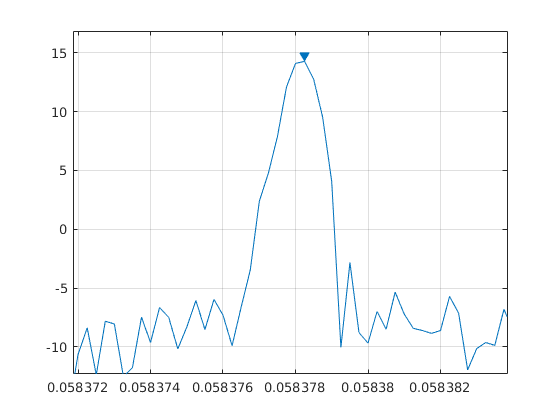
\includegraphics[width=0.5\textwidth,height=3cm]{closewinb2ex1.png}}
% \caption{N-signals experimental result from LFM BW of $2 MHz$ (left) and BW of $1 MHz$ (right)}
% \label{fig:lfmnlfm}
% \end{figure}
% \FloatBarrier
% The n-signal scheme also works with more diverse signals such as LFM and Frank P4 polyphase, Figure \ref{fig:lfmnp4}. The signals extracted from received signal are clearly affected by the other waveform, the extracted signals from the received is focused on the pattern to show how it is affected. This may have been the result of intermodulation distortion from SDR hardware nonlinearity.   Nevertheless, their matched filter result, Figure \ref{fig:lfmnp4mf} is still capable of detecting range from these signals. 
% \begin{figure}[h]
% \centering\makebox{
% \noindent\makebox{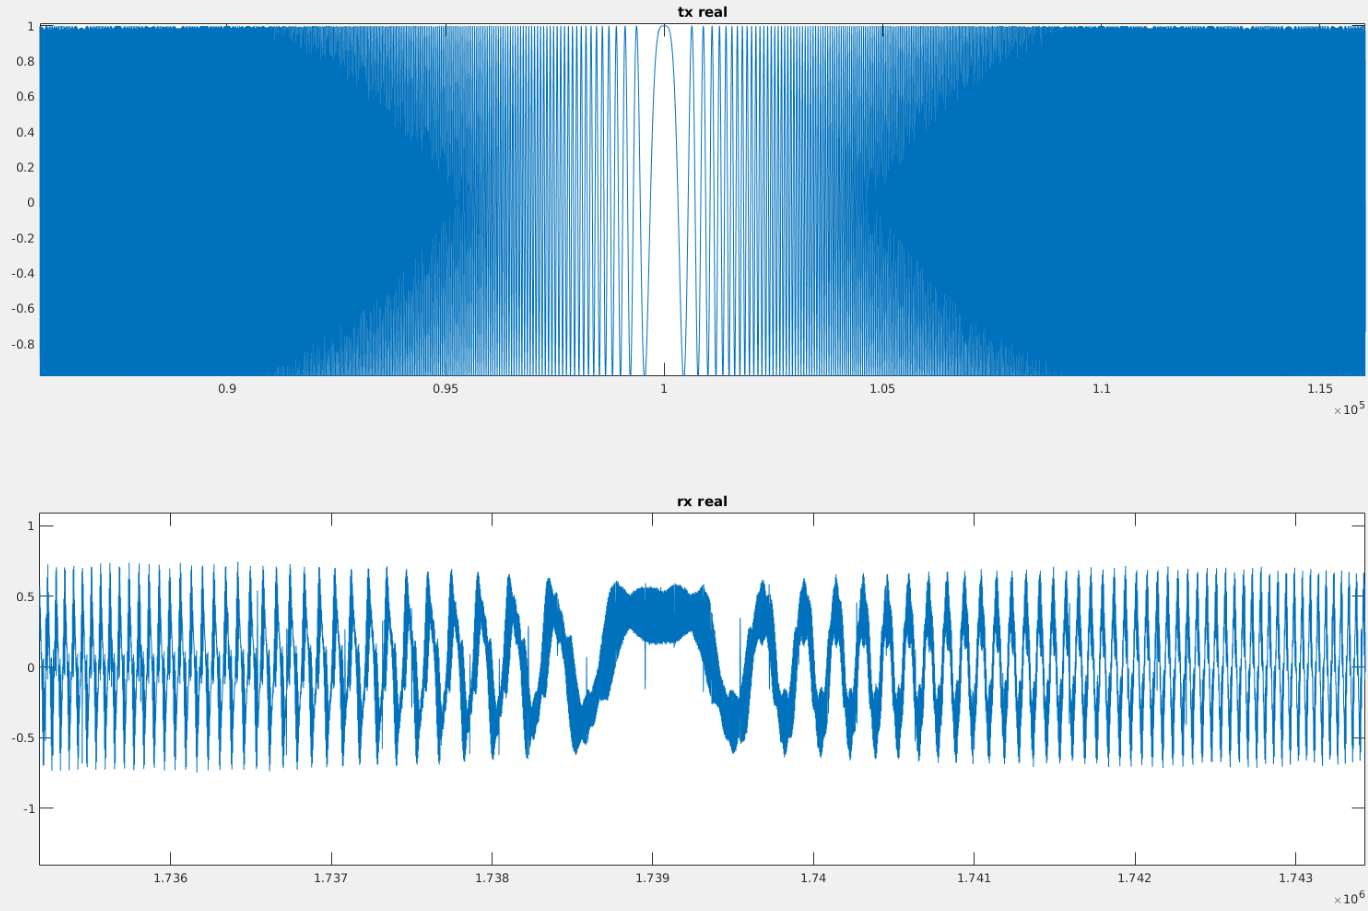
\includegraphics[width=0.4\textwidth]{lfmnp41.png}}
% \noindent\makebox{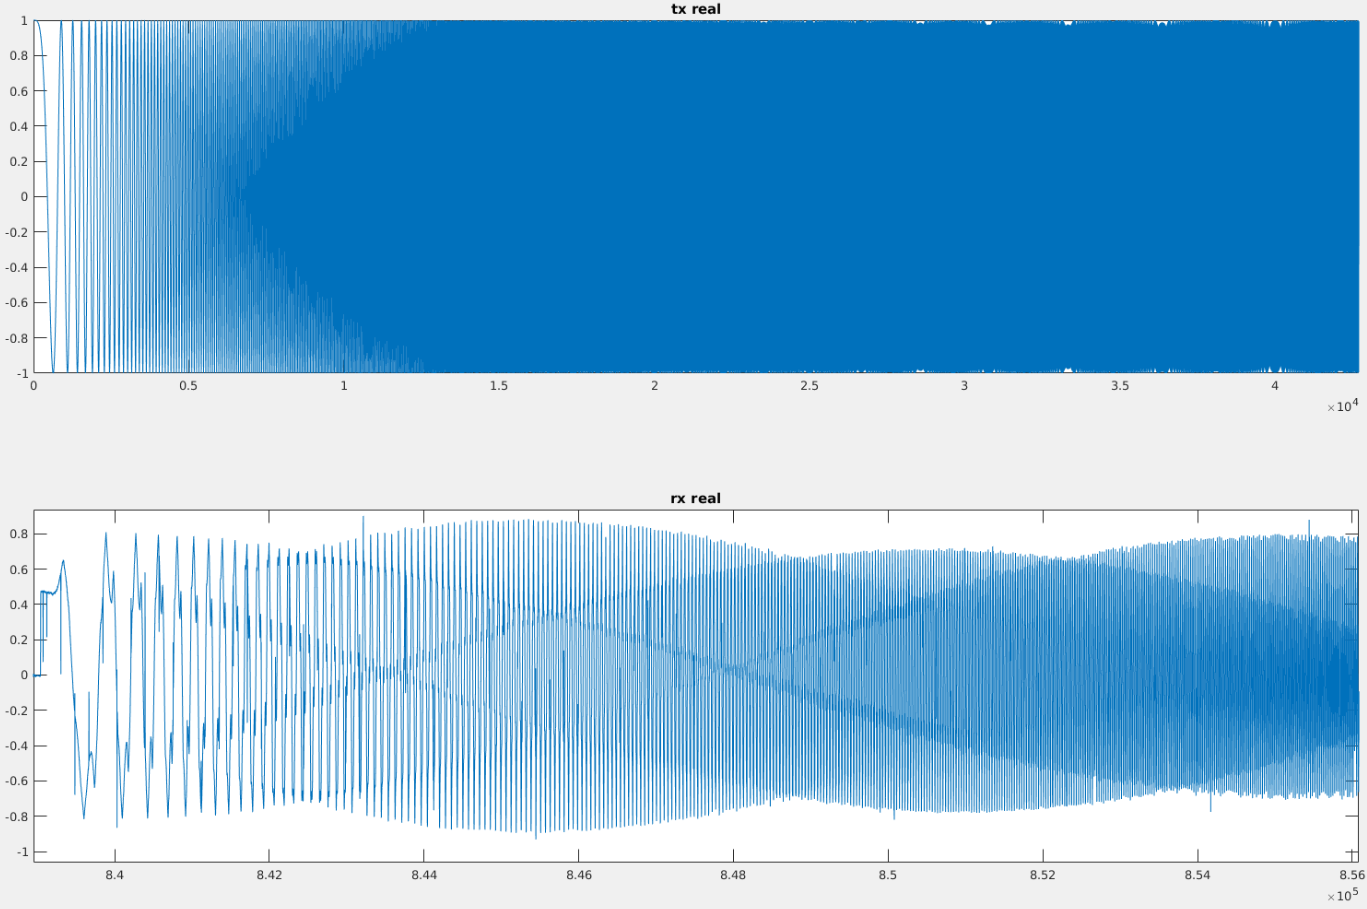
\includegraphics[width=0.4\textwidth]{lfmnp42.png}}}
% \caption{N-signals tranceiving signals from LFM (left) and Frank P4 polyphase (right)}
% \label{fig:lfmnp4}
% \end{figure}
% \begin{figure}[h]
% \noindent\makebox{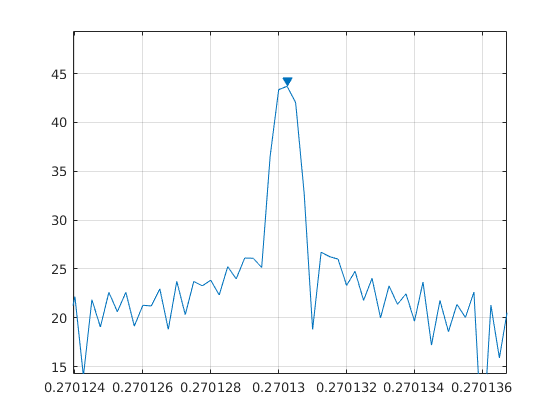
\includegraphics[width=0.5\textwidth,height=3cm]{p4nsig.png}}
% \noindent\makebox{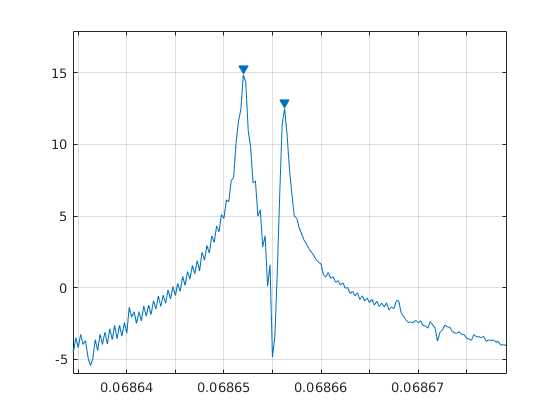
\includegraphics[width=0.5\textwidth,height=3cm]{lfmnsiglfmnsq.png}}
% \caption{N-signals matched filter result from LFM (left) and Frank P4 polyphase (right)}
% \label{fig:lfmnp4mf}
% \end{figure}
% \FloatBarrier
% The possible intermodulation distortion is enlarged when combining LFM with square pulse. This investigation, by comparing the same signal extraction that involves SDR Hardware and comparing it with extraction without the hardware involvement narrows the problem down to intermodulation as the primary distortion contributor. Figure \ref{fig:lfmnsq} shows the extracted square signal from combined signal went through USRP on the left and without USRP involvement on the right. 
% \begin{figure}[h]
% \noindent\makebox{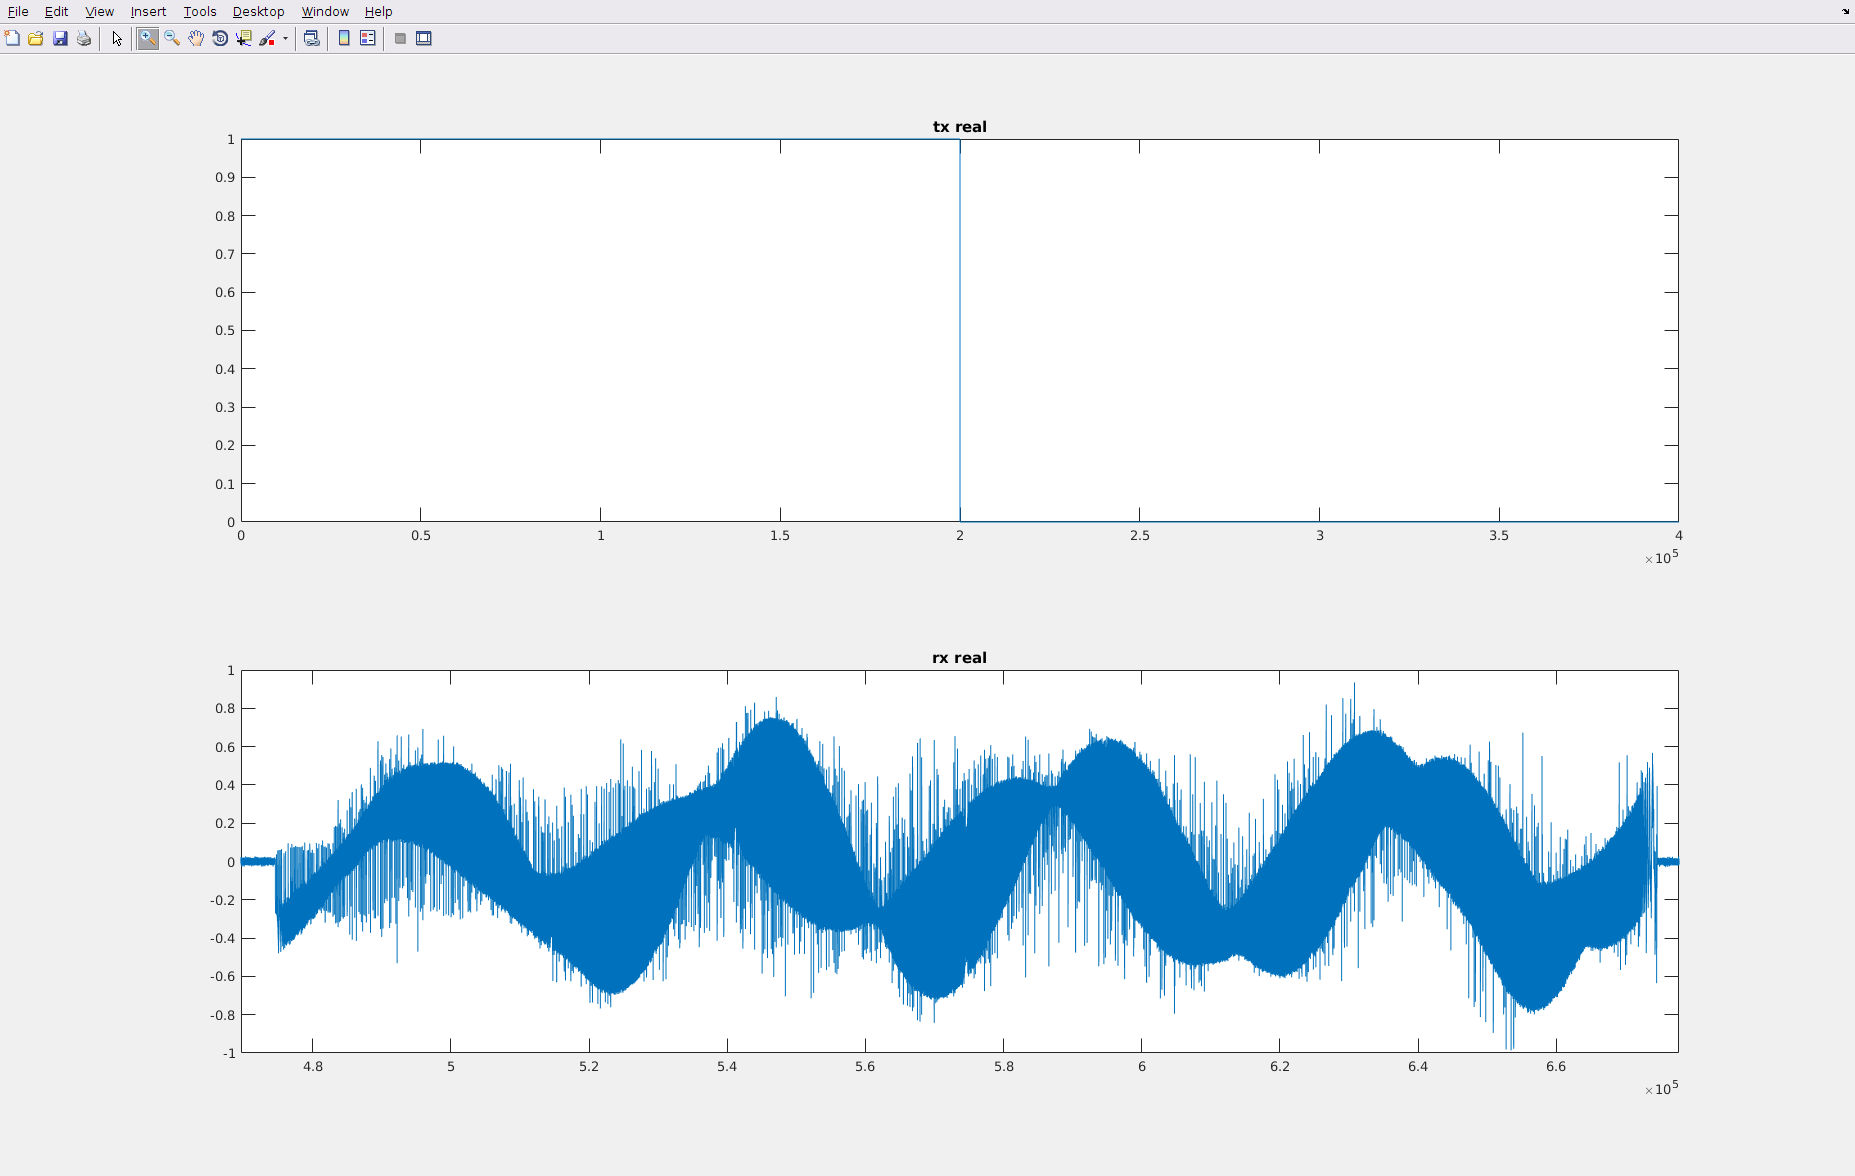
\includegraphics[width=0.5\textwidth]{sqrx.png}}
% \noindent\makebox{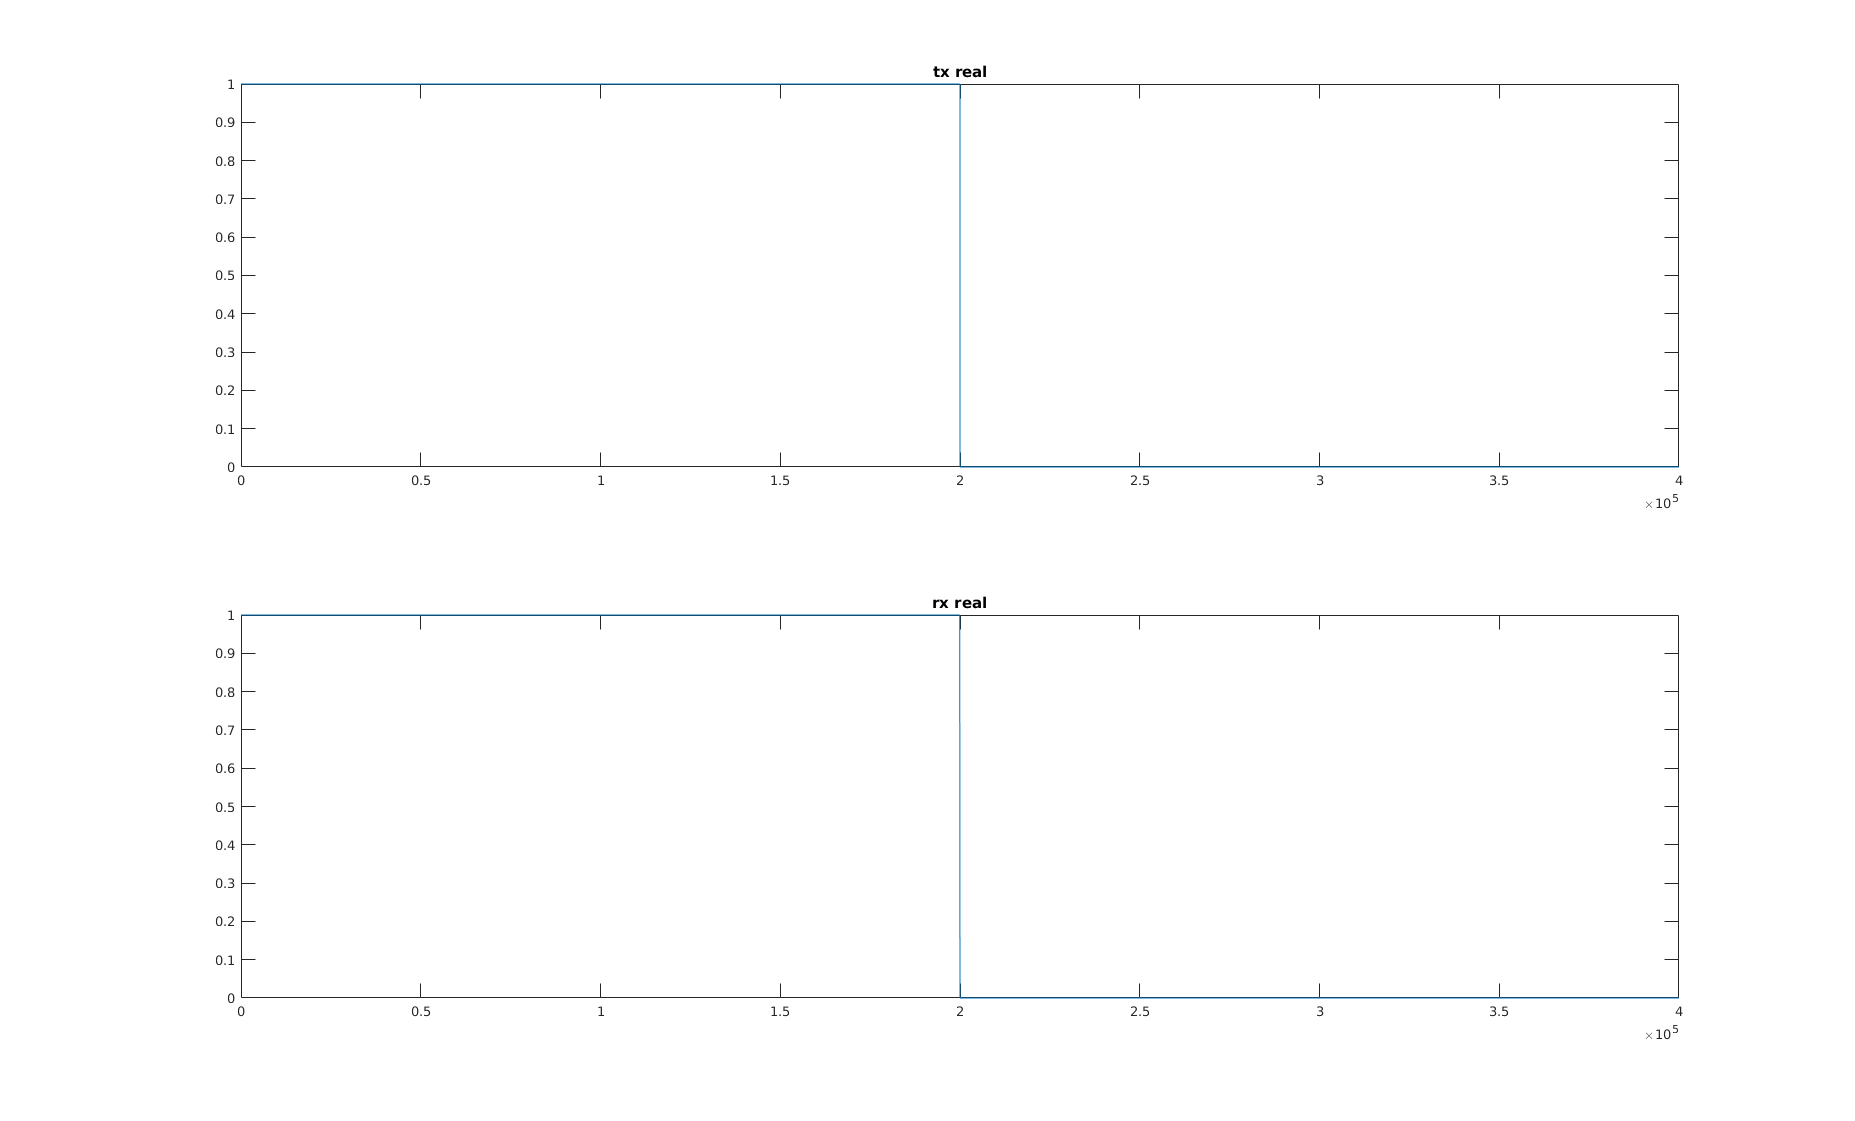
\includegraphics[width=0.5\textwidth]{sqsim.png}}
% \caption{Extracted square signal from n-signals scheme}
% \label{fig:lfmnsq}
% \end{figure}

% \FloatBarrier
% \section{Conclusion And Recommendation for Future Work}
% This project yields a new solution for portable inexpensive close ground airspace management. As an advanced solution choice than animal training or market control, the software Radar solution offers enough options for adapting to client purpose. There are still fair amount of work before product deployment; At this stage, it is ready to attract investment for ordering the Radar solution. The software solution is currently aiming for customers looking for specific setup instead of offering universal solution. In the future, with enough client requirements data for the types of Radar solution, a universal software Radar system will be available for immediate purchase. \\

% %-------------------------------------------------------------------------------
% % Recommendation and future work
% %-------------------------------------------------------------------------------
% The software product is currently built on high level programming language. With the general structure of the software ready, the recommended next move is to transfer current coding to C++ or other lower level language for faster live data processing. The current Radar system is not tested against multi-targets ranging or other Radar antennas. More rigorous testing should be performed with different Radar antennas and ranging situations to ensure ubiquitous compatibility of the system.

% \section*{Acknowledgments}
% The authors would like to acknowledge the suggestions of many people.

% \begin{appendices}
% \renewcommand{\thesection}{\Alph{section}}

% \section{Implementation Attempt on Simulink}
% \label{app:simuerror}
% The implementation on Simulink, provided perfect results in simulation and offers an easy to use programming interface, was not able to deliver good Radar range results due to time delay sensitivities. Simulink is a very user friendly platform and provides perfect image rendering for data visualization. It was chosen as the primary platform for developing, implementing, and LFM Radar algorithm for this project. However, the simulink block diagram relies entirely on the recently developed USRP block for communicating with USRP. The Simulink USRP block used for this project is a 2016b edition. Operations before and after the USRP block provides ideal results, the expected results could be observed in data analysis without the USRP block. Figure \ref{fig:simugen} shows the flow graph of the Simulink.\\
% \begin{figure}[h]
% \centering\makebox{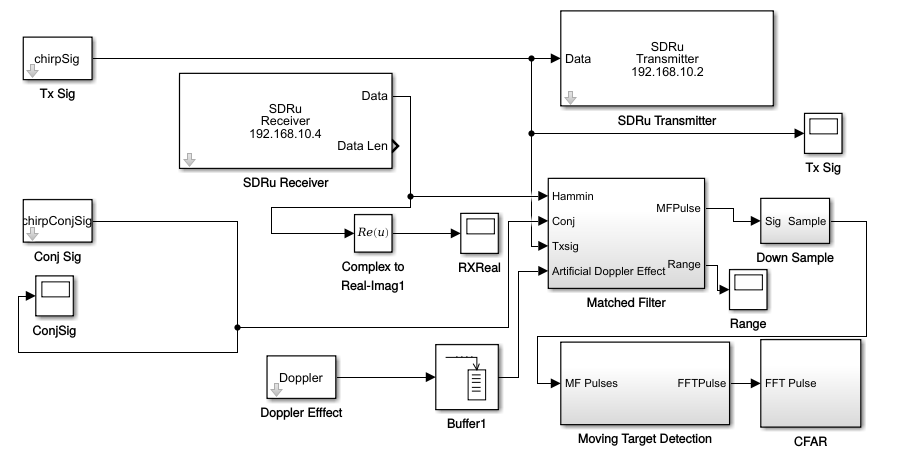
\includegraphics[width=0.5\textwidth]{simugen}}
% \caption{general view of Simulink block diagram}
% \label{fig:simugen}
% \end{figure}
% \FloatBarrier
% \subsection{Time Delay And Matched Filter}
% \label{app:tdmf}
% The important factor of Radar is to extract the time delay between the transmitted and received signal. This information could not be determined when passing the received signal through the matched filter algorithm. The matched filter algorithm has been extensively tested using simulated signals generated in MATLAB. Received signal is summation of reference signal and echo signal; both signal maintain the integrity of the transmitted signal with time delay shift in the echo signals. If time shift is less than sweep pulse width, in which echo signal reaches receiver before reference signal is done marking its time stamp, echo signal will be added to reference signal. The summation of the two signal will be the output of the receiver. The summation process is shown in Figure \ref{fig:sigadd}.\\
% \begin{figure}[h]
% \centering\makebox{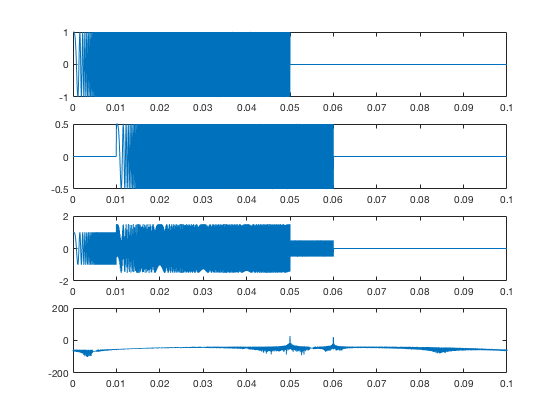
\includegraphics[width=0.5\textwidth]{sigadd}}
% \caption{reference, echo, and summation of the two signals}
% \label{fig:sigadd}
% \end{figure}
% Reference signal marks the time when the Radar signal is transmitted while echo signal is the one propagating to the target and reflects back to the receiver. In real Radar environment, sometimes the time delay would be far less than shown in Figure \ref{fig:sigadd} for near range targets. Figure \ref{fig:sig1dot2add} shows a simulated received signal with $1.2us$ time delay in between reference signal and echo signal which indicates a 360 meter free space distance. The time difference in this situation gives us a target that is near our Radar spatial resolution. Matched filter impulse response, shown at the bottom of Figure \ref{fig:sig1dot2add} , is displaying the exact time delay in between the two peaks.\\
% \begin{figure}[h]
% \centering\makebox{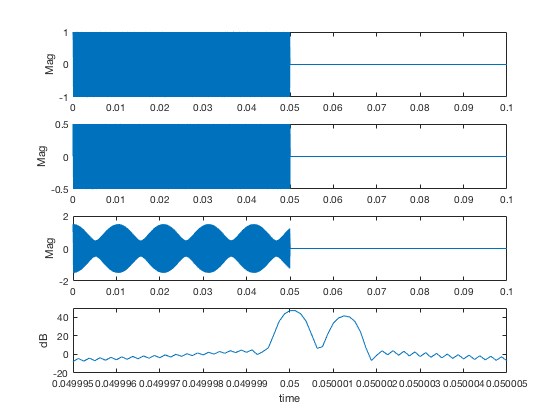
\includegraphics[width=0.5\textwidth]{sig1dot2add}}
% \caption{signals summation with $1.2us$ time delay between reference and echo signal and their matched filter response}
% \label{fig:sig1dot2add}
% \end{figure}
% \FloatBarrier
% \subsection{Minimum Detectable Range}
% \label{app:minDR}
% The spatial resolution determines the minimum amount of time delay a Radar can detect with its waveform specifications in LFM. A time delay between the signals will not show up on screen by matched filter algorithm once the time delay is below the spatial resolution which is also known as the bandwidth of impulse response from the matched filter. The matched filter bandwidth of the impulse response is determined by the bandwidth of LFM signal. The wider the LFM bandwidth the shorter the impulse response bandwidth. The exact relationship is displayed in Figure \ref{fig:bwrelation}. Top figures are displaying baseband chirp signal and bottom figures are their responsive matched filter impulse responses in time domain. The bandwidth of chirp signal will generate its matched filter impulse response with a new bandwidth of $\frac{2}{\textit{bandwidth of chirp signal}}$.\\

% \begin{figure}[h]
% \noindent\makebox{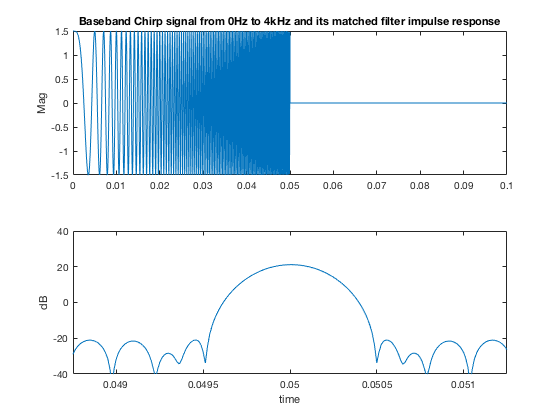
\includegraphics[width=0.5\textwidth]{bwrelation1}}
% \noindent\makebox{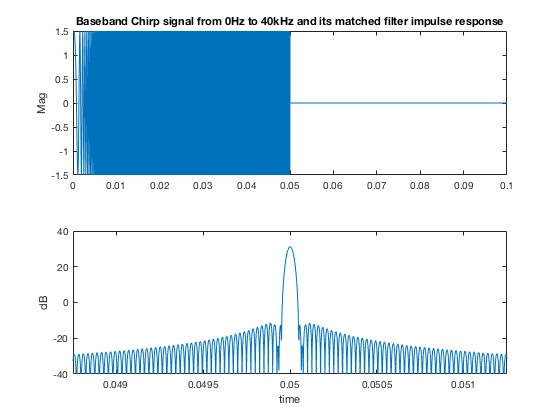
\includegraphics[width=0.5\textwidth]{bwrelation2}}
% \caption{Bandwidth of the LFM in relation with impulse response bandwidth}
% \label{fig:bwrelation}
% \end{figure}


% Figure \ref{fig:sig0dot5add} shows what happens to signals having equal and less time delay than what spatial resolution can handle and result in the impulse response unable to resolve two peaks for time delay calculation. On the left, the second peak is already joining the first peak, and on the right shows the second peak entirely merged with the reference peak and, thus, making time delay impossible to detect. \\



% \begin{figure}[h]
% \noindent\makebox{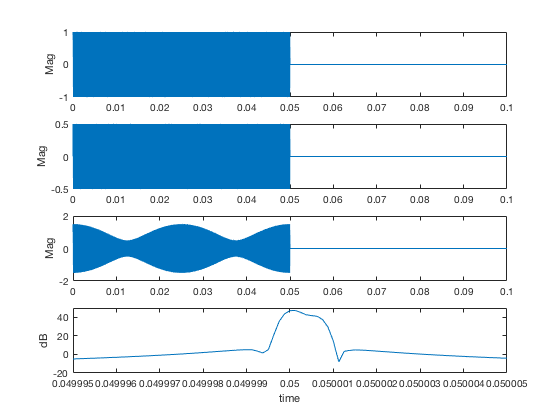
\includegraphics[width=0.5\textwidth]{sig0dot5add}}
% \noindent\makebox{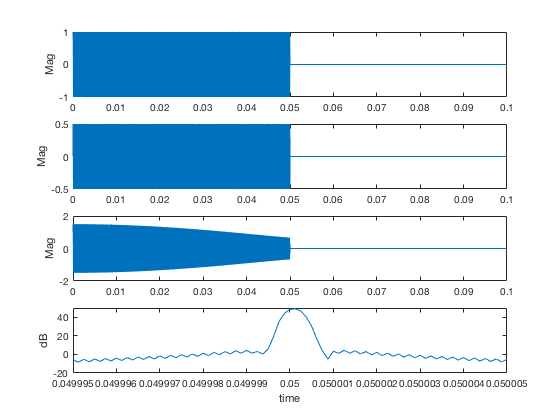
\includegraphics[width=0.5\textwidth]{sig0dot1add}}
% \caption{signals summation with $0.5us$ (left) and $0.1us$ (right) time delay between reference and echo signal and their matched filter response}
% \label{fig:sig0dot5add}
% \end{figure}

% While the Simulink USRP blocks respect the data integrity, the actual frequency of data transfer is disregarded. The simulation time does not match actual time , the resulting trade off is processing time. This particular problem does not show up in Simulink scopes as the receiver block restores the data. This was not apparent as the transceiving blocks are treated as black boxes in the setup. To display this problem, feed transmitted signal straight to the oscilloscope and focus on the sweeping time. From Simulink scope in Figure \ref{fig:simuoscitxcom} (left), the sweeping period matches the simulated time in this case is $0.2ms$ and $50\%$ duty cycle. However, on the oscilloscope, figure \ref{fig:simuoscitxcom} (right), the sweeping time period is,$8ms$, 40 time longer than what the Simulink scope indicates. This stretch in time is the result of time delay not shown on the data received by Simulink. The stretched sample rate is affecting the actual bandwidth of the signal causing the false second peak. The received signal from Simulink scope returns a regular looking signal with no sweeping time error, period of $0.2ms$ and $50\%$ duty cycle, as shown in Figure \ref{fig:simurx}, however, the time delay information is lost during the transition. \\
% \begin{figure}[H]
% \centering\makebox{
% \noindent\makebox{\includegraphics[width=0.4\textwidth]{simutxcom}}
% \noindent\makebox{\includegraphics[width=0.4\textwidth]{oscitxcom}}
% }
% \caption{transmitted chirp signal in Simulink scope (left) and oscilloscope (right)}
% \label{fig:simuoscitxcom}
% \end{figure}

% \begin{figure}[H]
% \centering\makebox{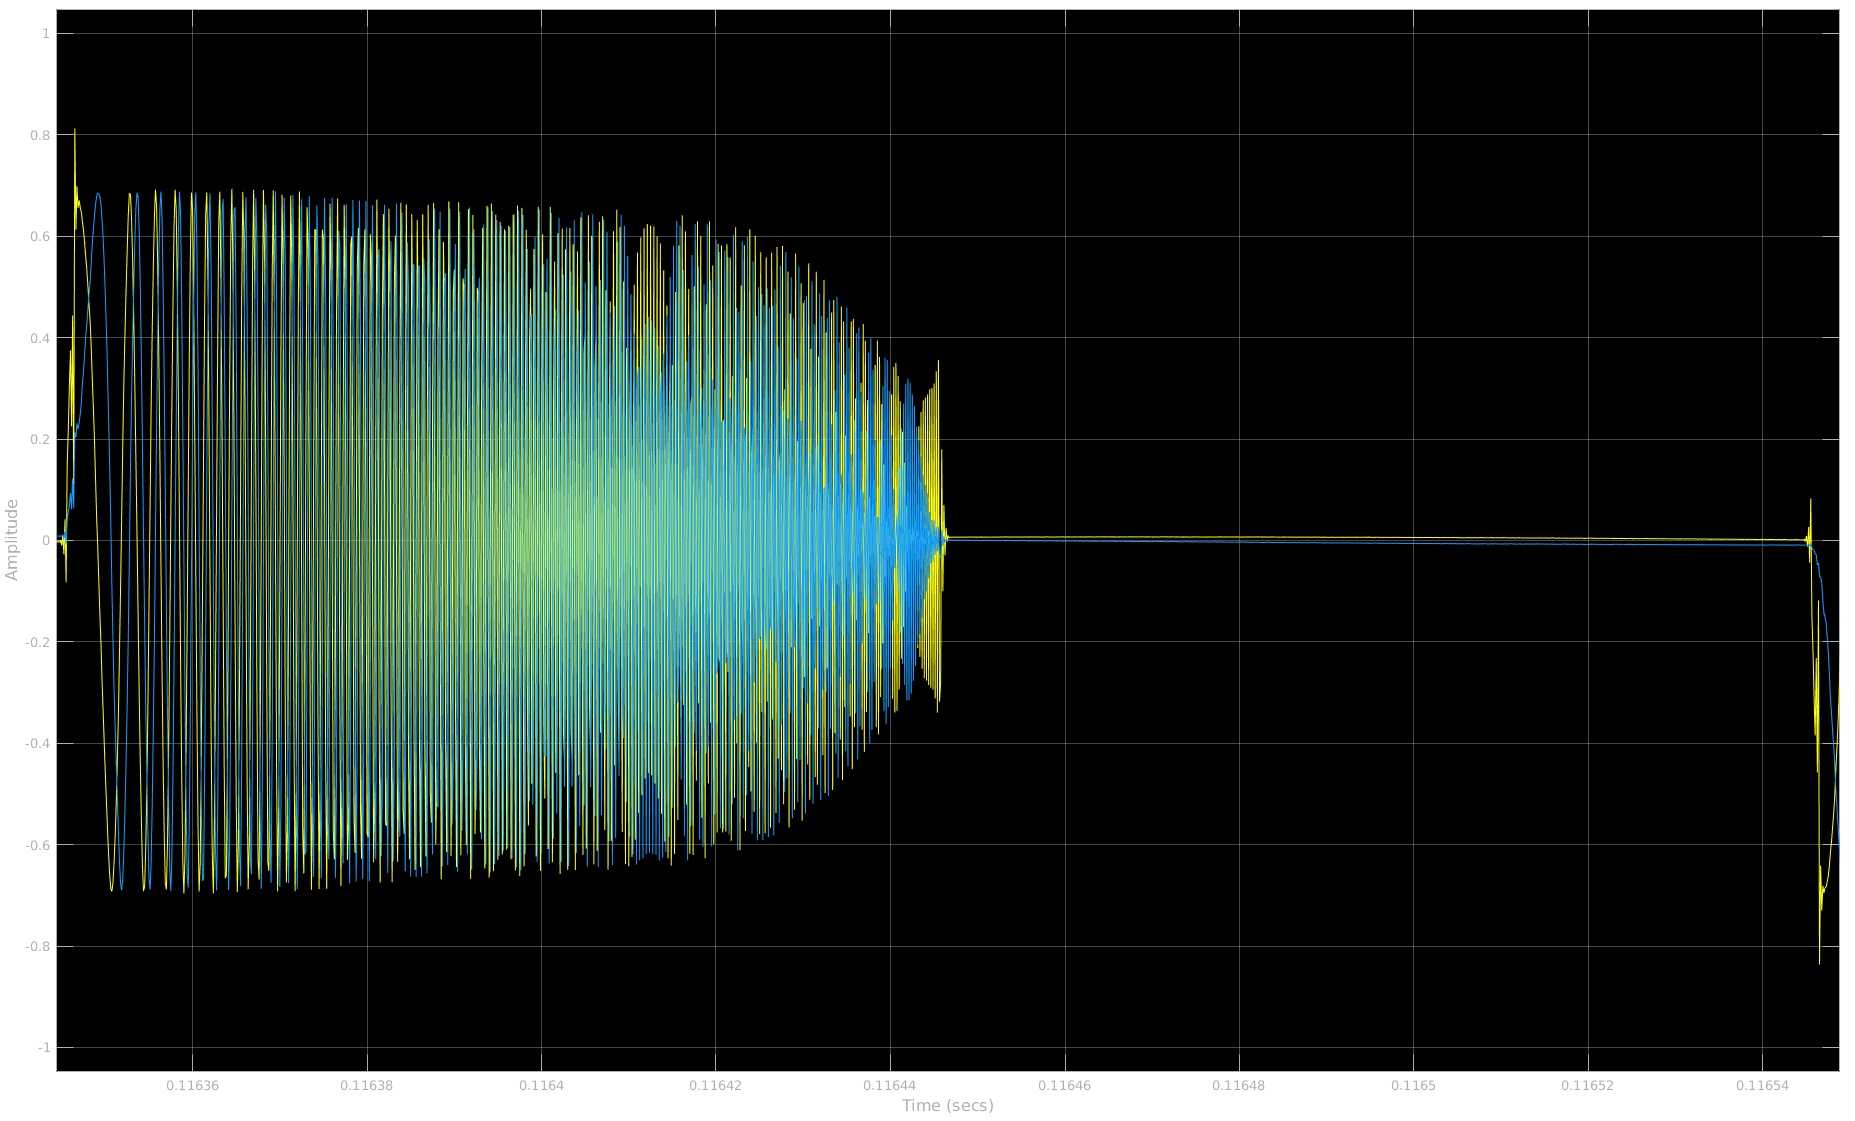
\includegraphics[width=0.5\textwidth]{rxrestore}}
% \caption{Simulink scope displaying received signal}
% \label{fig:simurx}
% \end{figure}

% In contrast, GNUradio is keeping sample time integrity which allowed success in this time delay sensitive experiment. Not only is the program respectful of the specified sample frequency, but is also capable of transmitting a large file size. This is shown in Figure \ref{fig:Gnu2Scopes} with same chirp signal, the left is the scope from GNUradio and right is from oscilloscope confirming its output is accurate.
% \begin{figure}[H]
% \centering\makebox{
% \noindent\makebox{\includegraphics[width=0.4\textwidth]{gnuscope}}
% \noindent\makebox{\includegraphics[width=0.415\textwidth]{ocilliscope}}
% }
% \caption{transmitted chirp signal in GNURadio scope (left) and oscilloscope (right)}
% \label{fig:Gnu2Scopes}
% \end{figure} 
% \end{appendices}

% \nocite{*}
% \bibliographystyle{IEEE}
% %%%%%\bibliography{bib-file}  % commented if *.bbl file included, as
% %%%%%see below


% %%%%%%%%%%%%%%%%% BIBLIOGRAPHY IN THE LaTeX file !!!!! %%%%%%%%%%%%%%%%%%%%%%%%
% %% This is nothing else than the IEEEsample.bbl file that you would         
% %%
% %% obtain with BibTeX: you do not need to send around the *.bbl file        
% %%
% %%---------------------------------------------------------------------------%%
% %
% \begin{thebibliography}{1}
% \bibitem{LaTeX}
% Leslie Lamport,
% \newblock {\em A Document Preparation System: \LaTeX, User's Guide and
%   Reference Manual},
% \newblock Addison Wesley Publishing Company, 1986.
% \bibitem{LaTeXD}
% Helmut Kopka,
% \newblock {\em \LaTeX, eine Einf\"uhrung},
% \newblock Addison-Wesley, 1989.
% \bibitem{TeX}
% D.K. Knuth,
% \newblock {\em The {\rm T\kern-.1667em\lower.7ex\hbox{E}\kern-.125emX}book},
% \newblock Addison-Wesley, 1989.
% \bibitem{METAFONT}
% D.E. Knuth,
% \newblock {\em The {\rm METAFONT}book},
% \newblock Addison Wesley Publishing Company, 1986.
% \end{thebibliography}
% %
% %%---------------------------------------------------------------------------%%

% \begin{biography}{Gerry Murray} will process your compu\-script,
% adding ``value'' to your \LaTeX\ file using a sophisticated text
% editor. Jeremy Barth will standardize the dimensions you've used, run
% a spell check, apply SGML tags to structure your document and validate
% all coding. The editor will ``on-screen edit'' the file, ``size'' your
% artwork and supply you with a laser proof by mail, or by fax, or even
% e-mail you a postscript version of the file which you can view on your
% workstation (using OpenWindows, NeXT, or an appropriate postscript
% viewer). When the editor is finished incorporating your amendments,
% Tom Bontrager, Mark Pheffer, Dalton Patterson or Chaucer Tran will
% receive the file and apply their abundant knowledge of typesetting to
% produce a document of the highest possible quality. A postscript file
% will be generated, output at 2032dpi on high quality RC paper for
% final examination by the editor. Christine will incorporate the
% artwork, the resulting camera-ready-copy will then be shot, the film
% supplied to the printer and your paper printed in the transaction for
% all to admire.
% \end{biography}

\end{document}

		
